% ================= CHAPTER 2 =================
\chapter{TINJAUAN PUSTAKA}

\section{Jarak/ Line Spacing}
Jarak baris dari bab ke sub bab adalah 3 lines. Jarak dari sub bab ke kalimat pertama adalah 1,5 lines.

\subsection{Sub-sub Bab}
Apabila sub-sub bab diperlukan, maka diketik dengan menggunakan garis bawah (\textit{underline}) namun tidak dicetak tebal. Penomorannya mengikuti sub bab seperti 2.1.1; 2.1.2; 2.1.3; dst.

\subsection{Sub-sub Bab}
Contoh penggunaan sub-sub bab lainnya.

\section{Persamaan}
Persamaan ditulis dengan menggunakan fitur equation pada M.S word dan menggunakan bantuan tabel. Contoh penulisan persamaan dapat dilihat pada persamaan 2.1.

\begin{equation}
    \rho = \frac{m}{V}
    \label{eq:rho}
\end{equation}

\section{Gambar}
Gambar dapat berupa foto atau grafik/skema yang dibutuhkan dalam penelitian dan menunjukkan keterkaitan dengan isi penelitian. Judul gambar dan grafik diletakkan di bawah objek dengan penomoran yang disesuaikan dengan babnya. Judul gambar yang hanya memerlukan 1 baris diketik dengan format rata tengah (\textit{centered}). Jika judul gambar memerlukan lebih dari satu baris, judul diketik dengan spasi 1 dengan format rata kanan-kiri (\textit{justify}), baris kedua atau lebih menyesuaikan indentasi huruf pertama judul gambar. Cetak tebal (\textit{bold}) digunakan untuk penulisan judul gambar. Karena judul gambar adalah suatu kalimat, maka diakhiri dengan titik. Umumnya, gambar diletakkan pada awal halaman atau pada bagian akhir halaman.

\begin{figure}[htbp]
    \centering
    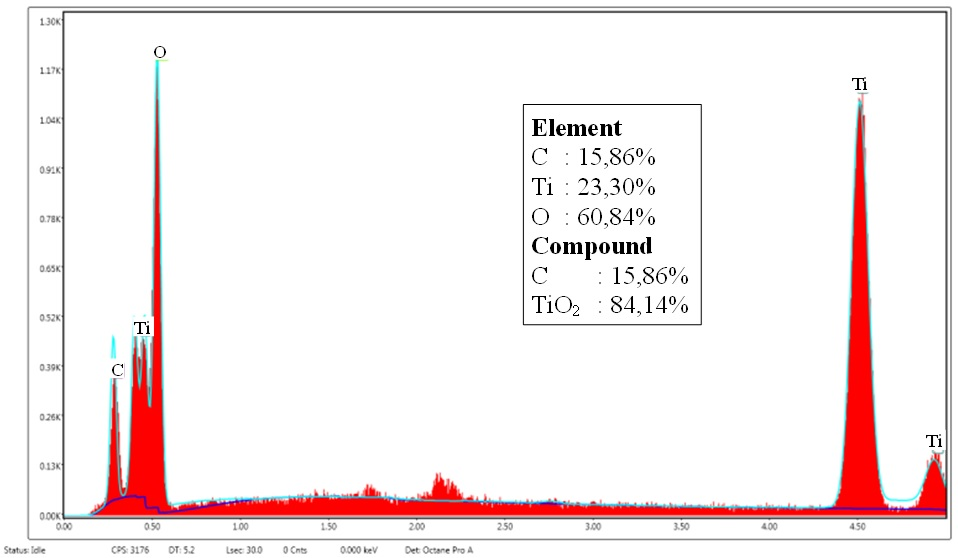
\includegraphics[width=0.6\textwidth]{assets/images/gambar_1}
    \caption{Spektrum EDS dari permukaan PP yang dilapisi TiO$_2$.}
    \label{fig:eds}
\end{figure}

Jika gambar dirujuk dalam narasi, maka huruf pertama pada kata ‘gambar’ ditulis dengan huruf besar (Gambar \ref{fig:eds}; Gambar \ref{fig:deposisi}; Gambar 4.3; dan seterusnya) walaupun berada di tengah kalimat. Contoh penyajian judul gambar yang memerlukan 1 baris dapat dilihat pada Gambar \ref{fig:eds}. Cara menuliskan judul gambar yang memerlukan lebih dari 1 baris disajikan pada Gambar \ref{fig:deposisi}.

\begin{figure}[htbp]
    \centering
    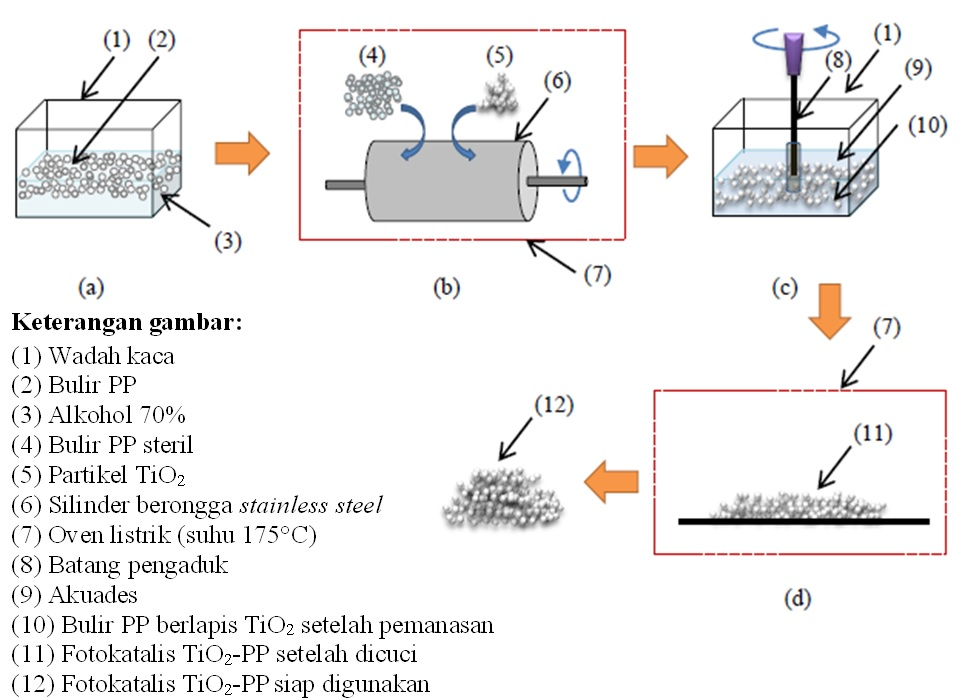
\includegraphics[width=0.6\textwidth]{assets/images/gambar_2}
    \caption{Deposisi TiO$_2$ pada permukaan PP dilakukan dengan (a) pembersihan bulir PP menggunakan alkohol 70\%, (b) imobilisasi TiO$_2$ pada permukaan PP dengan metode thermal milling untuk menghasilkan TiO$_2$-PP, (c) pembersihan TiO$_2$-PP, dan (d) pengeringan fotokatalis yang dihasilkan.}
    \label{fig:deposisi}
\end{figure}

\section{Tabel}
Tabel dibuat dengan garis horizontal saja tanpa garis vertikal. Ukuran huruf pada tabel diperbolehkan kurang dari 12 selama tulisannya masih jelas terbaca. Judul tabel diletakkan di atas objek dengan penomoran yang disesuaikan dengan babnya. Sama halnya dengan judul gambar, apabila judul tabel hanya memerlukan 1 baris diketik dengan format rata tengah (\textit{centered}). Jika judul tabel memerlukan lebih dari satu baris, judul diketik dengan spasi 1 dengan format rata kanan-kiri (\textit{justify}), baris kedua atau lebih menyesuaikan indentasi huruf pertama judul tabel. Berbeda halnya dengan cetak tebal (\textit{bold}) untuk penulisan judul gambar, judul tabel tidak dicetak tebal.

\begin{table}[htbp]
    \centering
    \caption{Laju deposisi \textit{thermal milling} untuk variasi waktu.}
    \begin{tabular}{ccc}
        \toprule
        Waktu milling (menit) & Massa TiO$_2$ terdeposisi (g) & Laju deposisi (mg/s) \\
        \midrule
        0 & 0 & 0,06 \\
        20 & 0,6 & 1,05 \\
        25 & 0,9 & 0,95 \\
        30 & 1,1 & 0,31 \\
        \bottomrule
    \end{tabular}
    \label{tab:milling}
\end{table}

Jika tabel dirujuk dalam narasi, maka huruf pertama pada kata ‘tabel’ ditulis dengan huruf besar (Tabel \ref{tab:milling}; Tabel \ref{tab:absorbansi}; Tabel 4.3; dst) walaupun berada di tengah kalimat. Contoh penyajian judul tabel yang memerlukan 1 baris dapat dilihat pada Tabel \ref{tab:milling}. Cara menuliskan judul tabel yang memerlukan lebih dari 1 baris disajikan pada Tabel \ref{tab:absorbansi}.

\begin{table}[htbp]
    \centering
    \caption{Nilai rata-rata absorbansi ($A$) sebagai fungsi waktu untuk setiap pengulangan penggunaan TiO$_2$-PP.}
    \begin{tabular}{ccccccc}
        \toprule
        Penggunaan ke- & \multicolumn{6}{c}{Nilai rata-rata $A$ setiap 8 jam (a.u)} \\
        \cmidrule(lr){2-7}
        & 0 jam & 8 jam & 16 jam & 24 jam & 32 jam & 40 jam \\
        \midrule
        1 & 2,89 & 1,637 & 1,217 & 1,130 & 0,154 & 0,154 \\
        2 & 2,89 & 1,559 & 1,522 & 0,546 & 0,186 & 0,15 \\
        3 & 2,89 & 1,645 & 1,272 & 0,630 & 0,154 & 0,156 \\
        4 & 2,89 & 1,602 & 1,340 & 1,326 & 0,225 & 0,206 \\
        5 & 2,89 & 1,644 & 1,586 & 1,400 & 0,916 & 0,465 \\
        \bottomrule
    \end{tabular}
    \label{tab:absorbansi}
\end{table}
